\documentclass[12pt, titlepage]{article}

\usepackage{amsmath, mathtools}

\usepackage[round]{natbib}
\usepackage{amsfonts}
\usepackage{amssymb}
\usepackage{graphicx}
\usepackage{colortbl}
\usepackage{xr}
\usepackage{hyperref}
\usepackage{longtable}
\usepackage{xfrac}
\usepackage{tabularx}
\usepackage{float}
\usepackage{siunitx}
\usepackage{booktabs}
\usepackage{multirow}
\usepackage[section]{placeins}
\usepackage{caption}
\usepackage{fullpage}

\hypersetup{
bookmarks=true,     % show bookmarks bar?
colorlinks=true,       % false: boxed links; true: colored links
linkcolor=red,          % color of internal links (change box color with linkbordercolor)
citecolor=blue,      % color of links to bibliography
filecolor=magenta,  % color of file links
urlcolor=cyan          % color of external links
}

\usepackage{array}

\externaldocument{../../SRS/SRS}

%% Comments

\usepackage{color}

\newif\ifcomments\commentstrue %displays comments
%\newif\ifcomments\commentsfalse %so that comments do not display

\ifcomments
\newcommand{\authornote}[3]{\textcolor{#1}{[#3 ---#2]}}
\newcommand{\todo}[1]{\textcolor{red}{[TODO: #1]}}
\else
\newcommand{\authornote}[3]{}
\newcommand{\todo}[1]{}
\fi

\newcommand{\wss}[1]{\authornote{blue}{SS}{#1}} 
\newcommand{\plt}[1]{\authornote{magenta}{TPLT}{#1}} %For explanation of the template
\newcommand{\an}[1]{\authornote{cyan}{Author}{#1}}

%% Common Parts

\newcommand{\progname}{ProgName} % PUT YOUR PROGRAM NAME HERE
\newcommand{\authname}{Team \#, Team Name
\\ Student 1 name
\\ Student 2 name
\\ Student 3 name
\\ Student 4 name} % AUTHOR NAMES                  

\usepackage{hyperref}
    \hypersetup{colorlinks=true, linkcolor=blue, citecolor=blue, filecolor=blue,
                urlcolor=blue, unicode=false}
    \urlstyle{same}
                                


\begin{document}

\title{Module Interface Specification for \progname{}}

\author{\authname}

\date{\today}

\maketitle

\pagenumbering{roman}

\section{Revision History}

\begin{tabularx}{\textwidth}{p{3cm}p{2cm}X}
  \toprule {\bf Date} & {\bf Version} & {\bf Notes}                                      \\
  \midrule
  Jan 3, 2024         & 1.0           & Added MIS for TeamT, GameT, PlayerT, Backend     \\
  Jan 14, 2024        & 1.1           & Added MIS for Season and Standing Record Modules \\
  Jan 17, 2024        & 1.2           & Added sections 2,3,4                             \\
  Apr 4, 2025         & 1.3           & Rev1 Revisions From Feedback                     \\
  \bottomrule
\end{tabularx}

~\newpage

\section{Symbols, Abbreviations and Acronyms}

See SRS Documentation at \url{https://github.com/dcheung11/team-6-capstone-project/blob/main/docs/SRS-Volere/SRS.pdf}

\renewcommand{\arraystretch}{1.2}
\begin{tabular}{l l}
  \toprule
  \textbf{symbol} & \textbf{description}                \\
  \midrule
  AC              & Anticipated Change                  \\
  DAG             & Directed Acyclic Graph              \\
  M               & Module                              \\
  MG              & Module Guide                        \\
  MIS             & Module Interface Specification      \\
  OS              & Operating System                    \\
  R               & Requirement                         \\
  SRS             & Software Requirements Specification \\
  UC              & Unlikely Change                     \\
  RBAC            & Role-Based Access Control           \\
  JSON            & JavaScript Object Notation          \\
  API             & Application Programming Interface   \\
  \bottomrule
\end{tabular}\\

\newpage

\tableofcontents

\newpage

\pagenumbering{arabic}

\section{Introduction}

The following document details the Module Interface Specifications for
Pitch Perfect McMaster GSA Softball League Platform. The platform is a web-based application designed to streamline league management. It enables users to create and join teams, schedule and reschedule games, track standings, and manage player rosters. With features like automated scheduling, announcements, and preferences for game timings, the platform simplifies league operations for players, captains, and administrators.

Complementary documents include the System Requirement Specifications
and Module Guide.  The full documentation and implementation can be
found at \url{https://github.com/dcheung11/team-6-capstone-project}.

\section{Notation}

The structure of the MIS for modules comes from \citet{HoffmanAndStrooper1995},
with the addition that template modules have been adapted from
\cite{GhezziEtAl2003}.  The mathematical notation comes from Chapter 3 of
\citet{HoffmanAndStrooper1995}.  For instance, the symbol := is used for a
multiple assignment statement and conditional rules follow the form $(c_1
  \Rightarrow r_1 | c_2 \Rightarrow r_2 | ... | c_n \Rightarrow r_n )$.

The following table summarizes the primitive data types used by \progname.

\begin{center}
  \renewcommand{\arraystretch}{1.2}
  \noindent
  \begin{tabular}{l l p{7.5cm}}
    \toprule
    \textbf{Data Type}  & \textbf{Notation} & \textbf{Description}                                             \\
    \midrule
    character           & char              & a single symbol or digit                                         \\
    integer             & $\mathbb{Z}$      & a number without a fractional component in (-$\infty$, $\infty$) \\
    natural number      & $\mathbb{N}$      & a number without a fractional component in [1, $\infty$)         \\
    real                & $\mathbb{R}$      & any number in (-$\infty$, $\infty$)                              \\
    multiple assignment & :=                & multiple assignment statement                                    \\
    set                 & $\{$ ... $\}$     & collection of unique elements                                    \\
    not in set          & $\backslash$      & element not in set                                               \\
    union               & $\cup$            & union of two sets                                                \\
    intersection        & $\cap$            & intersection of two sets                                         \\
    \bottomrule
  \end{tabular}
\end{center}

\noindent
The specification of \progname \ uses some derived data types: sequences, strings, and
tuples. Sequences are lists filled with elements of the same data type. Strings
are sequences of characters. Tuples contain a list of values, potentially of
different types. In addition, \progname \ uses functions, which
are defined by the data types of their inputs and outputs. Local functions are
described by giving their type signature followed by their specification.

\section{Module Decomposition}

The following table is taken directly from the Module Guide document for this project.

\begin{table}[h!]
  \centering
  \begin{tabular}{p{0.3\textwidth} p{0.6\textwidth}}
    \toprule
    \textbf{Level 1}                                      & \textbf{Level 2}              \\
    \midrule

    {Hardware-Hiding Module}                              & ~                             \\
    \midrule

    \multirow{7}{0.3\textwidth}{Behaviour-Hiding Module}  & User Interface Module         \\
                                                          & Authentication Module         \\
                                                          & Team Management Module        \\
                                                          & Game Management Module        \\
                                                          & Announcements Module          \\
                                                          & Scheduling Module             \\
                                                          & Standings Module              \\
                                                          & Waiver Module                 \\
                                                          & PlayerT Module                \\
                                                          & TeamT Module                  \\
                                                          & GameT Module                  \\
    \midrule

    \multirow{3}{0.3\textwidth}{Software Decision Module} & {Database Module}             \\
                                                          & {Notification Module}         \\
                                                          & {Scheduling Algorithm Module} \\
    \bottomrule
  \end{tabular}
  \caption{Module Hierarchy}
  \label{TblMH}
\end{table}

\newpage

\bibliographystyle {plainnat}
\bibliography {../../../refs/References}

\newpage

\section{MIS of User Interface Module (M1)} \label{Module:UI}

\subsection{Module}

User Interface Module

\subsection{Uses}

\begin{itemize}
  \item Backend Module: To retrieve and send data for rendering views and processing user inputs.
  \item Authentication Module: For user login and role verification.
  \item Game Management Module: To display and update game information.
  \item Team Management Module: To display team information
  \item Scheduling Module: To display schedules
  \item Standings Module: To display league standings and updates.
  \item Announcements Module: To display Announcements
  \item Notification Module: To display interface for creating notifications
\end{itemize}

\subsection{Syntax}

\subsubsection{Exported Constants}

\begin{itemize}
  \item None
\end{itemize}

\subsubsection{Exported Access Programs}

\begin{center}
  \begin{tabularx}{\textwidth}{|l|X|X|X|}
    \hline
    \textbf{Name} & \textbf{In} & \textbf{Out} & \textbf{Exceptions}  \\
    \hline
    renderView    & View        & -            & InvalidViewException \\
    \hline
  \end{tabularx}
\end{center}

\subsection{Semantics}

\subsubsection{State Variables}

\begin{itemize}
  \item \textbf{currentView}: Stores the identifier for the currently displayed view.
  \item \textbf{userRole}: Stores the role of the currently logged-in user (e.g., player, captain, commissioner).
\end{itemize}

\subsubsection{Environment Variables}

\begin{itemize}
  \item Browser environment: The module interacts with the user's browser, including DOM manipulation and event handling.
  \item Network connection: Required for fetching and sending data to the backend.
\end{itemize}

\subsubsection{Assumptions}

\begin{itemize}
  \item Users will have a modern web browser that supports the required JavaScript features.
  \item A stable network connection is available during interactions requiring backend communication.
\end{itemize}

\subsubsection{Access Routine Semantics}

\noindent \textbf{renderView(view)}:
\begin{itemize}
  \item transition: \texttt{currentView} := \texttt{view}.
  \item exception: Throws \texttt{InvalidViewException} if \texttt{view} is unsupported.
\end{itemize}

\subsubsection{Local Functions}
\begin{itemize}
  \item None
\end{itemize}

\section{MIS of Scheduling Module} \label{SchedulingModule}

\subsection{Module}
\textbf{Scheduling Module}: Behaviour-Hiding Module

\subsection{Uses}
\begin{itemize}
  \item Scheduling Algorithm Module
  \item TeamT Module
  \item GameT Module
\end{itemize}

\subsection{Syntax}

\subsubsection{Exported Constants}

\begin{itemize}
  \item \textbf{DEFAULT\_WEEK\_COUNT: Integer} \\ Default number of weeks in the season.
\end{itemize}

\subsubsection{Exported Access Programs}
\begin{center}
  \begin{tabular}{|p{4cm}| p{4cm}| p{4cm} | p{3cm}|}
    \hline
    \textbf{Name}   & \textbf{In}                     & \textbf{Out}    & \textbf{Exceptions}        \\
    \hline
    create schedule & TeamT[], Slot Object[], Integer & Schedule Object & -                          \\
    addGame         & GameT                           & Boolean         & InvalidInput               \\
    removeGame      & String                          & Boolean         & GameNotFound               \\
    updateGameSlot  & String, GameslotT               & Boolean         & GameNotFound               \\
    rescheduleGame  & String, GameT, GameT            & Boolean         & GameNotFound, SlotNotFound \\
    \hline
  \end{tabular}
\end{center}

\subsection{Semantics}

\subsubsection{State Variables}
\[
  \text{schedule} \subseteq \mathcal{T} \times \mathcal{S} \times \mathcal{G}
\]
where:
\begin{itemize}
  \item \(\mathcal{T}\): Set of all teams.
  \item \(\mathcal{S}\): Set of available slots.
  \item \(\mathcal{G}\): Set of all game identifiers.
\end{itemize}

\subsubsection{Environment Variables}
None.

\subsubsection{Assumptions}
\begin{itemize}
  \item \( \forall t \in \mathcal{T}, \; \exists s \in \mathcal{S}, \; t\) is scheduled exactly once per week.
  \item Valid team (\(t \in \mathcal{T}\)) and slot (\(s \in \mathcal{S}\)) data are provided for schedule creation.
\end{itemize}

\subsubsection{Access Routine Semantics}

\noindent \textbf{createSchedule(teams, slots, seasonLength):}
\begin{align*}
   & \text{transition: } \text{schedule} := \text{generateSchedule}(teams, slots, seasonLength)                     \\
   & \text{output: } \text{out} := \text{schedule}                                                                  \\
   & \text{constraint: } \forall t \in \mathcal{T}, \; \exists s \in \mathcal{S}, \; t \text{ plays once per week.} \\
   & \text{exception: } \text{None.}
\end{align*}

\vspace{1em}

\noindent \textbf{addGame(details):}
\begin{align*}
   & \text{transition: } \text{schedule} := \text{schedule} \cup \{(t_1, t_2, s) \;|\; t_1, t_2 \in \mathcal{T}, \; t_1 \neq t_2, \; s \in \mathcal{S}\} \\
   & \text{output: } \text{out} := \text{true if details are valid, false otherwise.}                                                                    \\
   & \text{exception: } \text{InvalidInput if details are incomplete or invalid.}
\end{align*}

\vspace{1em}

\noindent \textbf{removeGame(gameId):}
\begin{align*}
   & \text{transition: } \text{schedule} := \text{schedule} \setminus \{g \;|\; g \in \mathcal{G}, \; g.\text{id} = \text{gameId}\} \\
   & \text{output: } \text{out} := \text{true if gameId exists in schedule, false otherwise.}                                       \\
   & \text{exception: } \text{GameNotFound if gameId does not exist.}
\end{align*}

\vspace{1em}

\noindent \textbf{updateGameSlot(gameId, newSlot):}
\begin{align*}
   & \text{transition: } \text{schedule} := \text{schedule} \setminus \{g \;|\; g \in \mathcal{G}, \; g.\text{id} = \text{gameId}\} \\
   & \quad \cup \{(t_1, t_2, \text{newSlot})\}                                                                                      \\
   & \text{output: } \text{out} := \text{true if the update is successful.}                                                         \\
   & \text{exception: } \text{GameNotFound if gameId does not exist.}
\end{align*}

\vspace{1em}

\noindent \textbf{rescheduleGame(gameId, newSlot, oldSlot):}
\begin{align*}
   & \text{transition: } \text{schedule} := \text{schedule} \setminus \{(t_1, t_2, \text{oldSlot}) \;|\; t_1, t_2 \in \mathcal{T}\} \\
   & \quad \cup \{(t_1, t_2, \text{newSlot})\}                                                                                      \\
   & \text{output: } \text{out} := \text{true if the reschedule is successful.}                                                     \\
   & \text{exceptions: }
  \begin{cases}
    \text{GameNotFound} & \text{if gameId does not exist.}             \\
    \text{SlotNotFound} & \text{if oldSlot or newSlot does not exist.}
  \end{cases}
\end{align*}

\subsubsection{Local Functions}
None.


\newpage

\section{MIS of PlayerT Module} \label{PlayerTModule}

\subsection{Module}
\textbf{PlayerT}: Abstract Player Module.
\subsection{Uses}
TeamT
\begin{itemize}
  \item \textbf{GameT}: The Player module interacts with the Game module to track player participation in games.
  \item \textbf{TeamT}: The Player module is connected to the Team module, as players are assigned to teams.
\end{itemize}

\subsection{Syntax}

\subsubsection{Exported Constants}

\subsubsection{Exported Access Programs}

\begin{center}
  \begin{tabular}{|p{4cm}| p{4cm}| p{4cm} | p{3cm}|}
    \hline
    \textbf{Name}   & \textbf{In}                                  & \textbf{Out} & \textbf{Exceptions} \\
    \hline
    PlayerT         & String, String, String, String, Bool, String & -            & -                   \\
    getPlayerId     &                                              & String       & -                   \\
    getName         &                                              & String       & -                   \\
    getEmail        &                                              & String       & -                   \\
    getWaiverStatus &                                              & Bool         & -                   \\
    getTeam         &                                              & Bool         & -                   \\
    setWaiverStatus & Bool                                         & -            & -                   \\
    setTeam         & String                                       & -            & -                   \\
    \hline
  \end{tabular}
\end{center}

\subsection{Semantics}

\subsubsection{State Variables}
isLoggedIn: Boolean

\subsubsection{Environment Variables}
None

\subsubsection{Assumptions}
None

\subsubsection{Access Routine Semantics}

\noindent PlayerT(id, n, e, p, w, t):
\begin{itemize}
  \item transition: playerId, name, email, password, waiverStatus, team $:= \text{id}, n, e, p, w, t$
  \item output: out := self
  \item exception: None
\end{itemize}

\noindent getPlayerId():
\begin{itemize}
  \item output: out := playerId
  \item exception: None
\end{itemize}

\noindent getName():
\begin{itemize}
  \item output: out := name
  \item exception: None
\end{itemize}

\noindent getEmail():
\begin{itemize}
  \item output: out := email
  \item exception: None
\end{itemize}

\noindent getWaiverStatus():
\begin{itemize}
  \item output: out := waiverStatus
  \item exception: None
\end{itemize}

\noindent getTeam():
\begin{itemize}
  \item output: out := team
  \item exception: None
\end{itemize}

\noindent setTeam(t):
\begin{itemize}
  \item transition: team := t
  \item exception: None
\end{itemize}

\noindent setWaiverStatus(w):
\begin{itemize}
  \item transition: waiverStatus := w
  \item exception: None
\end{itemize}


\subsubsection{Local Functions}

\newpage

\section{MIS of GameT Module} \label{GameTModule}

\subsection{Module}
\textbf{GameT}: Abstract Game Type

\subsection{Uses}
TeamT

\subsection{Syntax}

\subsubsection{Exported Constants}

\subsubsection{Exported Access Programs}
\begin{center}
  \begin{tabularx}{\textwidth}{@{}lXlX@{}}
    \toprule
    \textbf{Name}           & \textbf{In}                                                             & \textbf{Out}     & \textbf{Exceptions}    \\
    \midrule
    \texttt{GameT}          & \texttt{String, String, Date, String, String, Integer, Integer, String} & --               & --                     \\
    \texttt{getGameId}      & --                                                                      & \texttt{String}  & --                     \\
    \texttt{getTeamsInGame} & --                                                                      & \texttt{TeamT[]} & \texttt{GameNotFound}  \\
    \texttt{getGameDetails} & --                                                                      & \texttt{Object}  & \texttt{GameNotFound}  \\
    \texttt{getStatus}      & --                                                                      & \texttt{String}  & \texttt{GameNotFound}  \\
    \texttt{getField}       & --                                                                      & \texttt{String}  & \texttt{GameNotFound}  \\
    \texttt{setStatus}      & \texttt{String}                                                         & --               & \texttt{InvalidStatus} \\
    \texttt{setField}       & \texttt{String}                                                         & --               & \texttt{InvalidField}  \\
    \texttt{setScore}       & \texttt{Integer, Integer}                                               & --               & \texttt{InvalidScore}  \\
    \bottomrule
  \end{tabularx}
\end{center}

\subsection{Semantics}

\subsubsection{State Variables}

\subsubsection{Environment Variables}
None

\subsubsection{Assumptions}
\begin{itemize}
  \item A game must have two teams assigned to it.
  \item A game must have a field assigned to it.
  \item A game's score can only be updated after the game is completed.
  \item The game status must be updated to reflect its current state (e.g., scheduled, completed).
\end{itemize}

\subsubsection{Access Routine Semantics}

\noindent GameT(id, t1, t2, d, t, s1, s2, f):
\begin{itemize}
  \item transition: gameId, team1Id, team2Id, gameDate, gameTime, scoreTeam1, scoreTeam2, field := id, t1, t2, d, t, s1, s2, f
  \item output: out := self
  \item exception: None
\end{itemize}

\noindent getGameId():
\begin{itemize}
  \item output: out := gameId
  \item exception: None
\end{itemize}

\noindent getGameDetails():
\begin{itemize}
  \item output: out := \text{Object containing game details: } gameId, team1Id, team2Id, gameDate, gameTime, scoreTeam1, scoreTeam2, status, field
  \item exception: Game not found if the game ID does not exist.
\end{itemize}

\noindent getTeamsInGame():
\begin{itemize}
  \item output: out := \text{Array of Teams participating in the game}
  \item exception: Game not found if the game ID does not exist.
\end{itemize}

\noindent getStatus():
\begin{itemize}
  \item output: out := status
  \item exception: Game not found if the game ID does not exist.
\end{itemize}

\noindent getField():
\begin{itemize}
  \item output: out := field
  \item exception: Game not found if the game ID does not exist.
\end{itemize}

\noindent setStatus(status):
\begin{itemize}
  \item transition: status := status
  \item exception: Invalid status if the provided status is not valid.
\end{itemize}

\noindent setField(field):
\begin{itemize}
  \item transition: field := field
  \item exception: Invalid field if the provided field is not valid.
\end{itemize}

\noindent setScore(score1, score2):
\begin{itemize}
  \item transition: scoreTeam1 := score1, scoreTeam2 := score2
  \item exception: Invalid score if the provided scores are not valid integers.
\end{itemize}

\subsubsection{Local Functions}
\begin{itemize}
  \item \textbf{validateGameDetails()}: A function to validate the input details when creating a new game.
\end{itemize}

\section{MIS of TeamT Module} \label{TeamModule}

\subsection{Module}
\textbf{TeamT Module}: Abstract Team Module

\subsection{Uses}
PlayerT, GameT

\subsection{Syntax}

\subsubsection{Exported Constants}

\subsubsection{Exported Access Programs}

\begin{center}
  \begin{tabular}{p{4cm} p{4cm} p{4cm} p{3cm}}
    \toprule
    \textbf{Name}         & \textbf{In}                                         & \textbf{Out}       & \textbf{Exceptions}     \\
    \midrule
    \texttt{TeamT}        & \texttt{String, String, String, PlayerT[], PlayerT} & -                  & -                       \\
    \texttt{getTeamId}    & -                                                   & \texttt{String}    & -                       \\
    \texttt{getTeamName}  & -                                                   & \texttt{String}    & -                       \\
    \texttt{getDivision}  & -                                                   & \texttt{String}    & -                       \\
    \texttt{getRoster}    & -                                                   & \texttt{PlayerT[]} & -                       \\
    \texttt{getCaptain}   & -                                                   & \texttt{PlayerT}   & -                       \\
    \texttt{addPlayer}    & \texttt{PlayerT}                                    & -                  & \texttt{InvalidPlayer}  \\
    \texttt{removePlayer} & \texttt{PlayerT}                                    & -                  & \texttt{PlayerNotFound} \\
    \bottomrule
  \end{tabular}
\end{center}


\subsection{Semantics}

\subsubsection{State Variables}

\subsubsection{Environment Variables}
None

\subsubsection{Assumptions}
\begin{itemize}
  \item Each team must have a unique team ID.
  \item A team can belong to one division at a time.
  \item The team roster must be an array or list of players (with unique player identifiers).
\end{itemize}

\subsubsection{Access Routine Semantics}

\noindent TeamT(id, n, d, r, c):
\begin{itemize}
  \item transition: teamId, teamName, division, roster, captain := id, n, d, r, c
  \item output: out := self
  \item exception: None
\end{itemize}

\noindent getTeamId():
\begin{itemize}
  \item output: out := teamId
  \item exception: None
\end{itemize}

\noindent getTeamName():
\begin{itemize}
  \item output: out := teamName
  \item exception: None
\end{itemize}

\noindent getDivision():
\begin{itemize}
  \item output: out := division
  \item exception: None
\end{itemize}

\noindent getRoster():
\begin{itemize}
  \item output: out := roster
  \item exception: None
\end{itemize}

\noindent getCaptain():
\begin{itemize}
  \item output: out := captain
  \item exception: None
\end{itemize}

\noindent addPlayer(player):
\begin{itemize}
  \item transition: roster := roster + player
  \item exception: Invalid player if the player is invalid or already in the roster.
\end{itemize}

\noindent removePlayer(player):
\begin{itemize}
  \item transition: roster := roster - player
  \item exception: Player not found if the player is not in the roster.
\end{itemize}

\subsubsection{Local Functions}
None

\section{MIS of Backend Module} \label{Backend}

\subsection{Module}

Backend/Database

\subsection{Uses}
PlayerT, GameT, TeamT

\subsection{Syntax}

\subsubsection{Exported Constants}

\subsubsection{Exported Access Programs}

\begin{center}
  \begin{tabular}{p{4cm} p{4cm} p{4cm} p{4cm}}
    \toprule
    \textbf{Name}                 & \textbf{In}                                                             & \textbf{Out}       & \textbf{Exceptions}          \\
    \midrule
    \texttt{createPlayer}         & \texttt{String, String, String, String, Bool, String}                   & -                  & \texttt{PlayerCreationError} \\
    \texttt{getPlayer}            & \texttt{String}                                                         & \texttt{PlayerT}   & \texttt{PlayerNotFound}      \\
    \texttt{updatePlayer}         & \texttt{String, String, String, String, Bool, String}                   & -                  & \texttt{PlayerNotFound}      \\
    \texttt{deletePlayer}         & \texttt{String}                                                         & -                  & \texttt{PlayerNotFound}      \\
    \texttt{createTeam}           & \texttt{String, String, String, PlayerT[], PlayerT}                     & -                  & \texttt{TeamCreationError}   \\
    \texttt{getTeam}              & \texttt{String}                                                         & \texttt{TeamT}     & \texttt{TeamNotFound}        \\
    \texttt{updateTeam}           & \texttt{String, String, String, PlayerT[], PlayerT}                     & -                  & \texttt{TeamCreationError}   \\
    \texttt{deleteTeam}           & \texttt{String}                                                         & -                  & \texttt{TeamNotFound}        \\
    \texttt{createGame}           & \texttt{String, String, Date, String, String, Integer, Integer, String} & -                  & \texttt{GameCreationError}   \\
    \texttt{getGame}              & \texttt{String}                                                         & \texttt{GameT}     & \texttt{GameNotFound}        \\
    \texttt{updateGame}           & \texttt{String, String, Date, String, String, Integer, Integer, String} & -                  & \texttt{GameCreationError}   \\
    \texttt{deleteGame}           & \texttt{String}                                                         & -                  & \texttt{GameNotFound}        \\
    \texttt{getAllPlayersForTeam} & \texttt{String}                                                         & \texttt{PlayerT[]} & \texttt{TeamNotFound}        \\
    \texttt{getAllGamesForTeam}   & \texttt{String}                                                         & \texttt{GameT[]}   & \texttt{TeamNotFound}        \\
    \bottomrule
  \end{tabular}
\end{center}


\subsection{Semantics}

\subsubsection{State Variables}
None

\subsubsection{Environment Variables}
None

\subsubsection{Assumptions}

\begin{itemize}
  \item The backend is connected to a database
  \item Each database operation (CRUD) will be encapsulated in a backend method to ensure separation of concerns
  \item Data consistency and integrity are maintained by the backend during each operation.
\end{itemize}

\subsubsection{Access Routine Semantics}

\noindent createPlayer(name, email, password, waiverStatus, team):
\begin{itemize}
  \item transition: playerId, name, email, password, waiverStatus, team := name, email, password, waiverStatus, team
  \item exception: "Player Creation Error" if player cannot be created
\end{itemize}

\noindent getPlayer(playerId):
\begin{itemize}
  \item output: out := player (retrieves player object based on playerId)
  \item exception: "Player Not Found" if player does not exist
\end{itemize}

\noindent updatePlayer(playerId, name, email, password, waiverStatus, team):
\begin{itemize}
  \item transition: name, email, password, waiverStatus, team := name, email, password, waiverStatus, team (updates player's details)
  \item exception: "Player Not Found" if player does not exist
\end{itemize}

\noindent deletePlayer(playerId):
\begin{itemize}
  \item transition: player := null (deletes the player from the database)
  \item exception: "Player Not Found" if player does not exist
\end{itemize}

\noindent createTeam(teamName, division, captain, roster):
\begin{itemize}
  \item transition: teamId, teamName, division, captain, roster := teamName, division, captain, roster
  \item exception: "Team Creation Error" if team cannot be created
\end{itemize}

\noindent getTeam(teamId):
\begin{itemize}
  \item output: out := team (retrieves team object based on teamId)
  \item exception: "Team Not Found" if team does not exist
\end{itemize}

\noindent updateTeam(teamId, teamName, division, roster):
\begin{itemize}
  \item transition: teamName, division, roster := teamName, division, roster (updates team's details)
  \item exception: "Team Not Found" if team does not exist
\end{itemize}

\noindent deleteTeam(teamId):
\begin{itemize}
  \item transition: team := null (deletes the team from the database)
  \item exception: "Team Not Found" if team does not exist
\end{itemize}

\noindent createGame(teams, date, time, field, score):
\begin{itemize}
  \item transition: gameId, teams, date, time, field, score := teams, date, time, field, score (creates a new game)
  \item exception: "Game Creation Error" if game cannot be created (e.g., scheduling conflict)
\end{itemize}

\noindent getGame(gameId):
\begin{itemize}
  \item output: out := game (retrieves game object based on gameId)
  \item exception: "Game Not Found" if game does not exist
\end{itemize}

\noindent updateGame(gameId, updates):
\begin{itemize}
  \item transition: gameId, updates := gameId, updates (updates the game's details)
  \item exception: "Game Not Found" if game does not exist
\end{itemize}

\noindent deleteGame(gameId):
\begin{itemize}
  \item transition: game := null (deletes the game from the database)
  \item exception: "Game Not Found" if game does not exist
\end{itemize}

\noindent getAllPlayersForTeam(teamId):
\begin{itemize}
  \item output: out := players (retrieves all players associated with the team)
  \item exception: "Team Not Found" if team does not exist
\end{itemize}

\noindent getAllGamesForTeam(teamId):
\begin{itemize}
  \item output: out := games (retrieves all games associated with the team)
  \item exception: "Team Not Found" if team does not exist
\end{itemize}

\subsubsection{Local Functions}
None

\subsubsection{ERD for Database}
% see local file Capstone_ERD.png if better quality needed
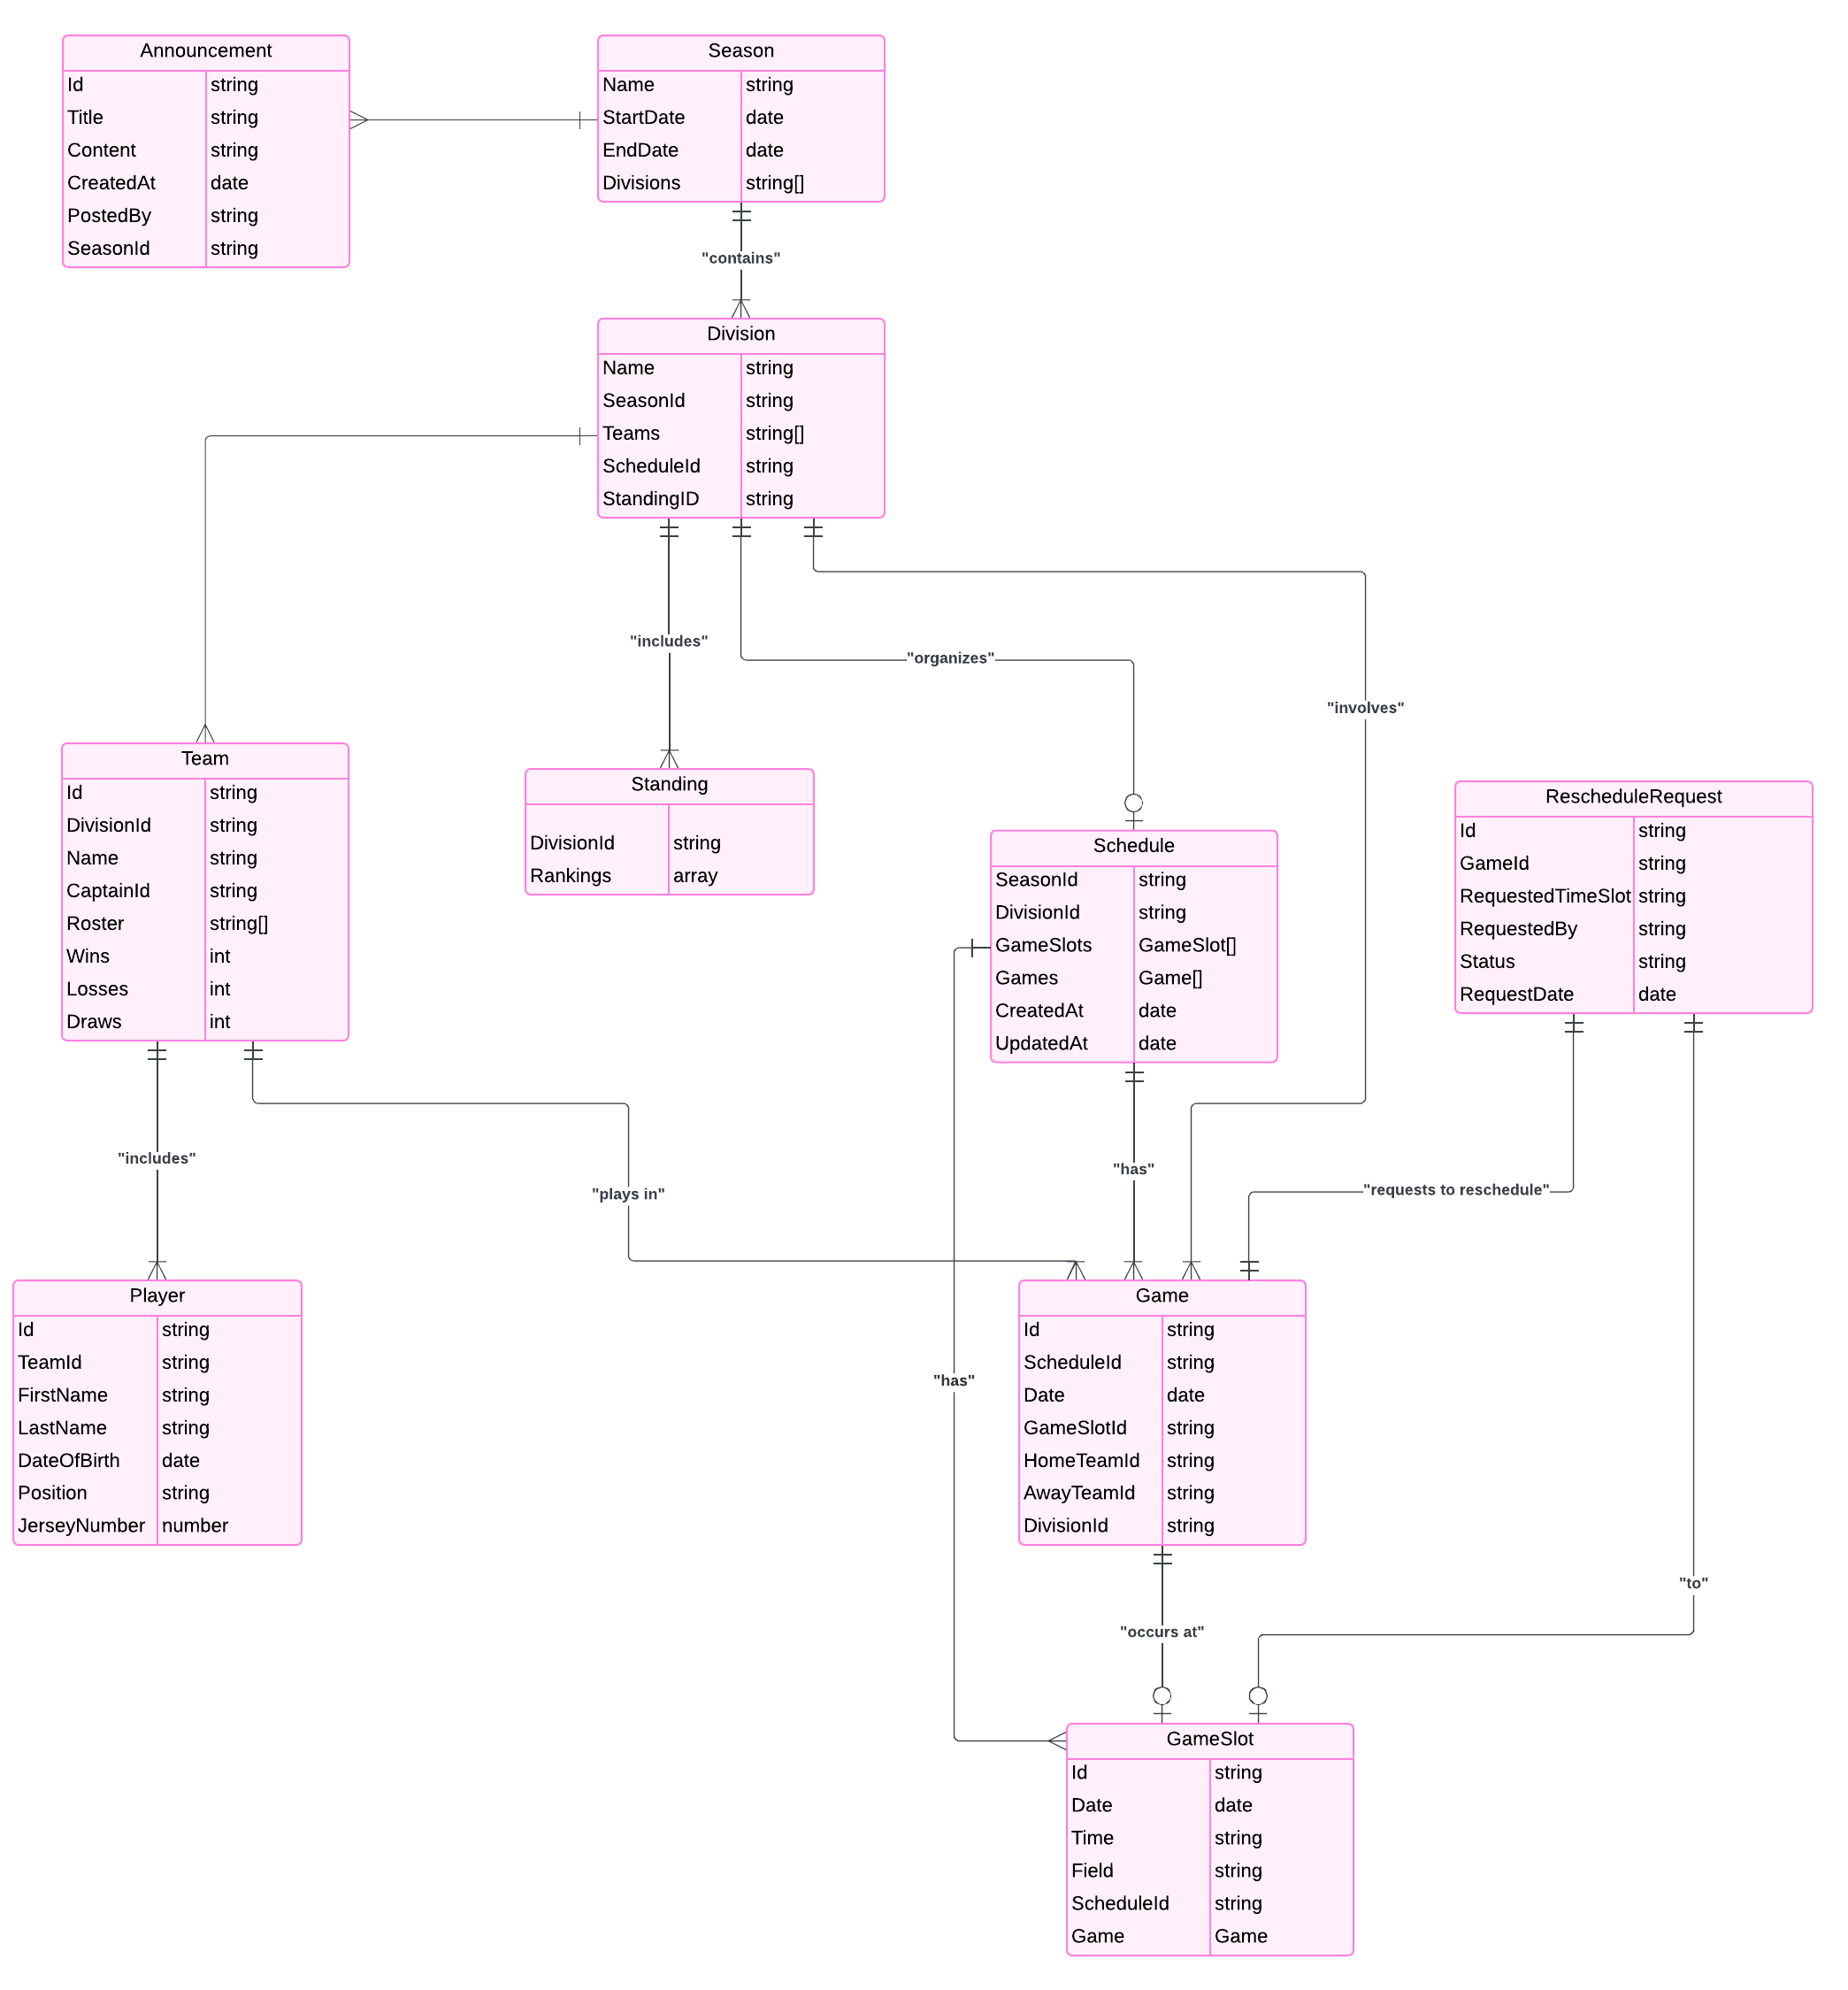
\includegraphics[scale=0.5]{Capstone_ERD.png}

\section{MIS of Waiver Module} \label{WaiverModule}

\subsection{Module}
Waiver

\subsection{Uses}

\begin{itemize}
  \item None
\end{itemize}

\subsection{Syntax}

\subsubsection{Exported Constants}
\begin{itemize}
  \item None
\end{itemize}

\subsubsection{Exported Access Programs}
\begin{center}
  \begin{tabular}{p{3cm} p{4cm} p{4cm} p{5cm}}
    \toprule
    \textbf{Name}         & \textbf{In}                 & \textbf{Out}             & \textbf{Exceptions}                                      \\
    \midrule
    \texttt{createWaiver} & \texttt{Waiver details}     & \texttt{Waiver ID}       & \texttt{InvalidInputException}                           \\
    \texttt{getWaiver}    & \texttt{Waiver ID}          & \texttt{Waiver details}  & \texttt{WaiverNotFoundException}                         \\
    \texttt{signWaiver}   & \texttt{User ID, Waiver ID} & \texttt{Boolean}         & \texttt{WaiverNotFoundException, AlreadySignedException} \\
    \texttt{listWaivers}  & \texttt{User ID}            & \texttt{List of waivers} & -                                                        \\
    \bottomrule
  \end{tabular}
\end{center}


\subsection{Semantics}

\subsubsection{State Variables}

\begin{itemize}
  \item \texttt{waiverList}: A collection of all waivers, including details and user signatures.
\end{itemize}

\subsubsection{Environment Variables}
\begin{itemize}
  \item Database: For storage of waiver details and signatures.
\end{itemize}

\subsubsection{Assumptions}
\begin{itemize}
  \item All users accessing the waiver module are authenticated.
  \item Waiver text complies with the legal requirements of the university softball league.
\end{itemize}

\subsubsection{Access Routine Semantics}

\noindent \texttt{createWaiver}(details):
\begin{itemize}
  \item transition: Adds a new waiver to \texttt{waiverList}.
  \item output: Returns a unique identifier for the created waiver.
  \item exception: Raises \texttt{InvalidInputException} if the waiver details are incomplete.
\end{itemize}

\noindent \texttt{getWaiver}(waiverID):
\begin{itemize}
  \item output: Retrieves details of the specified waiver.
  \item exception: Raises \texttt{WaiverNotFoundException} if the waiver does not exist.
\end{itemize}

\noindent \texttt{signWaiver}(playerID, waiverID):
\begin{itemize}
  \item transition: Updates \texttt{waiverList} to record the user's signature for the specified waiver.
  \item output: Returns \texttt{true} if the signature is successful.
  \item exception: Raises \texttt{WaiverNotFoundException} if the waiver does not exist or \texttt{AlreadySignedException} if the user has already signed the waiver.
\end{itemize}

\noindent \texttt{listWaivers}(userID):
\begin{itemize}
  \item output: Returns all waivers associated with the user.
\end{itemize}

\subsubsection{Local Functions}
\begin{itemize}
  \item None
\end{itemize}

\section{MIS of Notification Module} \label{Module:Notification}

\subsection{Module}

Notification

\subsection{Uses}

\begin{itemize}
  \item None
\end{itemize}

\subsection{Syntax}

\subsubsection{Exported Constants}

\begin{itemize}
  \item MAX\_NOTIFICATION\_LENGTH: Maximum allowed characters in a notification message.
  \item NOTIFICATION\_RETRY\_LIMIT: Maximum retry attempts for failed notifications.
\end{itemize}

\subsubsection{Exported Access Programs}

\begin{center}
  \begin{tabular}{p{2cm} p{4cm} p{4cm} p{4.5cm}}
    \toprule
    \textbf{Name}     & \textbf{In}                                       & \textbf{Out}     & \textbf{Exceptions}                            \\
    \midrule
    \texttt{send}     & \texttt{NotificationID}, \texttt{\text{playerID}} & \texttt{Boolean} & \texttt{InvalidPlayerID}, \texttt{SendFailure} \\
    \texttt{schedule} & \texttt{NotificationID}, \texttt{DateTime}        & \texttt{Boolean} & \texttt{InvalidDateTime}                       \\
    \texttt{status}   & \texttt{NotificationID}                           & \texttt{Status}  & \texttt{InvalidNotificationID}                 \\
    \bottomrule
  \end{tabular}
\end{center}


\subsection{Semantics}

\subsubsection{State Variables}

\begin{itemize}
  \item \texttt{pendingNotifications}: List of notifications yet to be delivered.
  \item \texttt{deliveredNotifications}: List of successfully delivered notifications.
\end{itemize}

\subsubsection{Environment Variables}

\begin{itemize}
  \item Email Gateway: For sending email notifications.
  \item SMS Gateway: For sending SMS notifications.
\end{itemize}

\subsubsection{Assumptions}

\begin{itemize}
  \item Users have valid email addresses or phone numbers stored in the database.
  \item Gateway APIs are operational and accessible.
\end{itemize}

\subsubsection{Access Routine Semantics}

\noindent \texttt{send}(NotificationID, playerID):
\begin{itemize}
  \item transition: Moves the notification from \texttt{pendingNotifications} to \texttt{deliveredNotifications} if successfully sent.
  \item output: \texttt{true} if the notification is successfully sent; \texttt{false} otherwise.
  \item exception: \texttt{InvalidPlayerID} if the playerID is not found; \texttt{SendFailure} if the notification fails to send after retries.
\end{itemize}

\noindent \texttt{schedule}(NotificationID, DateTime):
\begin{itemize}
  \item transition: Adds the notification to the \texttt{pendingNotifications} queue with the scheduled delivery time.
  \item output: \texttt{true} if the scheduling is successful; \texttt{false} otherwise.
  \item exception: \texttt{InvalidDateTime} if the DateTime is in the past or improperly formatted.
\end{itemize}

\noindent \texttt{status}(NotificationID):
\begin{itemize}
  \item transition: None.
  \item output: The status of the notification (e.g., Pending, Delivered, Failed).
  \item exception: \texttt{InvalidNotificationID} if the NotificationID is not found.
\end{itemize}

\subsubsection{Local Functions}

\begin{itemize}
  \item \texttt{validateNotification(NotificationID)}: Ensures the notification exists and is properly formatted.
  \item \texttt{retryFailedNotifications()}: Attempts to resend notifications marked as failed.
\end{itemize}

\newpage

\section{MIS of Authentication Module} \label{Auth}

\subsection{Module}

\textbf{Auth} (M2) - Abstract object for handling user authentication and session management.

\subsection{Uses}

\begin{itemize}
  \item \textbf{User Interface Module} (M1) - For collecting user credentials (username, password)
        and displaying authentication feedback.
  \item \textbf{Backend Module} (M13) - For verifying credentials, managing tokens, and storing
        authentication data.
\end{itemize}


\subsection{Syntax}

\subsubsection{Exported Constants}
\begin{itemize}
  \item \texttt{SESSION\_TIMEOUT} - Integer representing session timeout in minutes (default: 30).
\end{itemize}

\subsubsection{Exported Access Programs}

\begin{center}
  \begin{tabular}{|p{3cm} | p{4cm} | p{4cm} | p{4cm}|}
    \hline
    \textbf{Name}          & \textbf{In}            & \textbf{Out}   & \textbf{Exceptions}         \\
    \hline
    \texttt{login}         & String, String         & Boolean        & \texttt{InvalidCredentials} \\
    \texttt{logout}        & String                 & Void           & \texttt{SessionNotFound}    \\
    \texttt{registerUser}  & String, String, String & Boolean        & \texttt{DuplicateUserError} \\
    \texttt{verifyToken}   & String                 & Boolean        & \texttt{TokenExpiredError}  \\
    \texttt{generateToken} & String                 & String (Token) & \texttt{UserNotFound}       \\
    \hline
  \end{tabular}
\end{center}

\subsection{Semantics}

\subsubsection{State Variables}

\begin{itemize}
  \item \textbf{userSessions}: Map of active session tokens to user IDs.
  \item \textbf{userData}: Map of user IDs to credentials and roles.
\end{itemize}

\subsubsection{Environment Variables}

\begin{itemize}
  \item \textbf{Database Connection}: Used for storing and retrieving user authentication data.
  \item \textbf{SSL/TLS Connection}: Required for secure communication between client and server.
\end{itemize}

\subsubsection{Assumptions}

\begin{itemize}
  \item All passwords are stored as securely hashed values.
  \item Token expiration is managed based on \texttt{SESSION\_TIMEOUT}.
\end{itemize}

\subsubsection{Access Routine Semantics}

\begin{itemize}
  \item \texttt{login(username, password)}
        \begin{itemize}
          \item \textbf{Transition}: If the username and password match, generate a session token and add it to \texttt{userSessions}.
          \item \textbf{Output}: Returns \texttt{true} if successful, otherwise throws \texttt{InvalidCredentials}.
          \item \textbf{Exception}: Throws \texttt{InvalidCredentials} if the username or password is incorrect.
        \end{itemize}

  \item \texttt{logout(token)}
        \begin{itemize}
          \item \textbf{Transition}: Removes the token from \texttt{userSessions}.
          \item \textbf{Output}: None.
          \item \textbf{Exception}: Throws \texttt{SessionNotFound} if the token is invalid or expired.
        \end{itemize}

  \item \texttt{registerUser(username, password, role)}
        \begin{itemize}
          \item \textbf{Transition}: Adds a new entry to \texttt{userData} with hashed password and role.
          \item \textbf{Output}: Returns \texttt{true} if registration is successful.
          \item \textbf{Exception}: Throws \texttt{DuplicateUserError} if the username already exists.
        \end{itemize}

  \item \texttt{verifyToken(token)}
        \begin{itemize}
          \item \textbf{Output}: Returns \texttt{true} if the token is valid, otherwise throws \texttt{TokenExpiredError}.
          \item \textbf{Exception}: Throws \texttt{TokenExpiredError} if the token is expired.
        \end{itemize}

  \item \texttt{generateToken(userID)}
        \begin{itemize}
          \item \textbf{Output}: Generates a unique token linked to the \texttt{userID}.
          \item \textbf{Exception}: Throws \texttt{UserNotFound} if the user ID does not exist.
        \end{itemize}
\end{itemize}

\subsubsection{Local Functions}

\begin{itemize}
  \item \texttt{hashPassword(password)}: Converts a plaintext password into a securely hashed value.
  \item \texttt{validatePassword(inputPassword, storedHash)}: Compares an input password to the stored hashed password.
  \item \texttt{generateUniqueToken(userID)}: Generates a cryptographically secure token linked to a user ID.
\end{itemize}

\section{MIS of Team Management Module} \label{TeamManagementModule}

\subsection{Module}
Team Management

\subsection{Uses}
\begin{itemize}
  \item Waiver Module
  \item Notification Module
\end{itemize}

\subsection{Syntax}

\subsubsection{Exported Constants}
\begin{itemize}
  \item None
\end{itemize}

\subsubsection{Exported Access Programs}
\begin{center}
  \begin{tabular}{|p{3cm}|p{4cm}|p{4cm}|p{4cm}|}
    \hline
    \textbf{Name}           & \textbf{In}        & \textbf{Out} & \textbf{Exceptions}          \\
    \hline
    \texttt{createTeam}     & Team details       & Boolean      & InvalidInput                 \\
    \texttt{getTeamDetails} & Team ID            & String       & TeamNotFound                 \\
    \texttt{updateTeam}     & Team ID, Updates   & Boolean      & TeamNotFound                 \\
    \texttt{deleteTeam}     & Team ID            & Boolean      & TeamNotFound                 \\
    \texttt{listTeams}      & League ID          & List         & -                            \\
    \texttt{createPlayer}   & Team ID, Player ID & Boolean      & TeamNotFound                 \\
    \texttt{deletePlayer}   & Team ID, Player ID & Boolean      & TeamNotFound, PlayerNotFound \\
    \hline
  \end{tabular}
\end{center}

\subsection{Semantics}

\subsubsection{State Variables}
\begin{itemize}
  \item \texttt{teamList}: A collection of all teams, their details, and associated players.
  \item \texttt{leagueTeams}: A mapping between leagues and their associated teams.
\end{itemize}

\subsubsection{Environment Variables}
\begin{itemize}
  \item None
\end{itemize}

\subsubsection{Assumptions}
\begin{itemize}
  \item All team operations are initiated by authorized users.
  \item Team details such as names and IDs are unique within a league
\end{itemize}

\subsubsection{Access Routine Semantics}

\noindent \texttt{createTeam}(details):
\begin{itemize}
  \item transition: Adds a new team to \texttt{teamList}.
  \item output: Returns a unique identifier for the created team.
  \item exception: Raises \texttt{InvalidInput} if the team details are incomplete or violate constraints (e.g., duplicate team name).
\end{itemize}

\noindent \texttt{getTeamDetails}(teamID):
\begin{itemize}
  \item output: Retrieves the details of the specified team.
  \item exception: Raises \texttt{TeamNotFound} if the team does not exist.
\end{itemize}

\noindent \texttt{updateTeam}(teamID, updates):
\begin{itemize}
  \item transition: Updates the details of the specified team in \texttt{teamList}.
  \item output: Returns \texttt{true} if the update is successful.
  \item exception: Raises \texttt{TeamNotFound} if the team does not exist.
\end{itemize}

\noindent \texttt{deleteTeam}(teamID):
\begin{itemize}
  \item transition: Removes the specified team from \texttt{teamList}.
  \item output: Returns \texttt{true} if the deletion is successful.
  \item exception: Raises \texttt{TeamNotFound} if the team does not exist.
\end{itemize}

\noindent \texttt{listTeams}(leagueID):
\begin{itemize}
  \item output: Returns a list of all teams associated with the specified league.
\end{itemize}

\noindent \texttt{createPlayer}(teamID, playerID):
\begin{itemize}
  \item transition: Adds a player to the specified team in \texttt{teamList}.
  \item output: Returns \texttt{true} if the player is successfully added.
  \item exception: Raises \texttt{TeamNotFound} if the team does not exist
\end{itemize}

\noindent \texttt{deletePlayer}(teamID, playerID):
\begin{itemize}
  \item transition: Removes a player from the specified team in \texttt{teamList}.
  \item output: Returns \texttt{true} if the player is successfully removed.
  \item exception: Raises \texttt{TeamNotFound} if the team does not exist or \texttt{PlayerNotFound} if the player is not part of the team
\end{itemize}

\subsubsection{Local Functions}
\begin{itemize}
  \item None
\end{itemize}

\section{MIS of Announcements Module} \label{AnnouncementsModule}

\subsection{Module}
Announcements

\subsection{Uses}
\begin{itemize}
  \item Notification Module
  \item Backend Module

        \subsection{Syntax}

        \subsubsection{Exported Constants}
  \item \texttt{ANNOUNCEMENT\_TYPE\_INFO}: Constant for an informational announcement type.
\end{itemize}

\subsubsection{Exported Access Programs}
\begin{center}
  \begin{tabular}{p{4cm} p{4cm} p{3.5cm} p{4.5cm}}
    \toprule
    \textbf{Name}               & \textbf{In}                                                  & \textbf{Out}            & \textbf{Exceptions}                                   \\
    \midrule
    \texttt{sendAnnouncement}   & \texttt{Announcement} details (\texttt{text}, \texttt{type}) & \texttt{AnnouncementID} & \texttt{InvalidInput}                                 \\
    \texttt{updateAnnouncement} & \texttt{AnnouncementID}                                      & \texttt{Boolean}        & \texttt{AnnouncementNotFound}, \texttt{InvalidUpdate} \\
    \texttt{deleteAnnouncement} & \texttt{AnnouncementID}                                      & \texttt{Boolean}        & \texttt{AnnouncementNotFound}                         \\
    \bottomrule
  \end{tabular}
\end{center}

\subsection{Semantics}

\subsubsection{State Variables}
\begin{itemize}
  \item None
\end{itemize}

\subsubsection{Environment Variables}
\begin{itemize}
  \item None
\end{itemize}

\subsubsection{Assumptions}
\begin{itemize}
  \item All announcement operations (create, update, delete) are performed by authorized users only.
  \item Users will be notified of new or updated announcements based on their notification preferences.
\end{itemize}

\subsubsection{Access Routine Semantics}

\noindent \texttt{sendAnnouncement}(announcementID):
\begin{itemize}
  \item transition: Sends a notification about the specified announcement to subscribed users using send()
  \item output: Returns \texttt{true} if the notification was sent successfully.
  \item exception: Raises \texttt{AnnouncementNotFoundException} if the announcement does not exist.
\end{itemize}

\noindent \texttt{updateAnnouncement}(announcementID):
\begin{itemize}
  \item transition: Updates the details of the specified announcement
  \item output: Returns \texttt{true} if the update is successful.
  \item exception: Raises \texttt{AnnouncementNotFound} if the announcement does not exist
\end{itemize}

\noindent \texttt{deleteAnnouncement}(announcementID):
\begin{itemize}
  \item transition: Removes the specified announcement
  \item output: Returns \texttt{true} if the deletion is successful.
  \item exception: Raises \texttt{AnnouncementNotFound} if the announcementID does not exist.
\end{itemize}

\subsubsection{Local Functions}
\begin{itemize}
  \item None
\end{itemize}

\newpage

\section{MIS of Scheduling Algorithm Module} \label{SchedulingAlgorithmModule}

\subsection{Module}
SchedulingAlgorithm: Software Decision Module.

\subsection{Uses}
\begin{itemize}
  \item Scheduling Module
  \item TeamT
  \item GameslotT
  \item GameT
\end{itemize}

\subsection{Syntax}

\subsubsection{Exported Constants}
\begin{itemize}
  \item DEFAULT\_WEEK\_COUNT: Integer \\ Default number of weeks for scheduling.
  \item MAX\_GAMES\_PER\_TEAM: Integer \\ Maximum number of games per team.
  \item MIN\_GAMES\_PER\_TEAM: Integer \\ Minimum number of games per team.
\end{itemize}

\subsubsection{Exported Access Programs}

\begin{center}
  \begin{tabular}{|p{3cm}|p{3.5cm}|p{3.5cm}|p{5cm}|}
    \hline
    Name             & In                   & Out             & Exceptions                \\
    \hline
    generateSchedule & TeamT[], GameslotT[] & Schedule object & InvalidInput              \\
    resolveConflicts & Schedule Object      & Schedule Object & ConflictResolutionFailure \\
    optimizeSchedule & Schedule Object      & Schedule Object & OptimizationFailure       \\
    \hline
  \end{tabular}
\end{center}

\subsection{Semantics}

\subsubsection{State Variables}
None

\subsubsection{Environment Variables}
None

\subsubsection{Assumptions}
\begin{itemize}
  \item Inputs, such as the list of teams, slots, and week count, are valid and non-empty.
  \item Teams have all required properties, such as constraints and preferences.
  \item Slots are pre-validated and adhere to game capacity limits.
  \item Conflicts are identifiable based on provided rules (e.g., double bookings, unavailable fields).
\end{itemize}

\subsubsection{Access Routine Semantics}

\noindent generateSchedule(teams, slots, weekCount):
\begin{itemize}
  \item output: out := schedule \\ A schedule object generated based on team constraints, slot availability, and the given week count.
  \item exception: Raises InvalidInput if the input is incomplete or invalid.
\end{itemize}

\noindent resolveConflicts(schedule):
\begin{itemize}
  \item transition: Resolves scheduling conflicts.
  \item output: out := updated\_schedule.
  \item exception: Raises ConflictResolutionFailure if the conflicts cannot be resolved.
\end{itemize}

\noindent optimizeSchedule(schedule):
\begin{itemize}
  \item transition: Refines the input schedule to improve adherence to the specified metrics.
  \item output: out := optimized\_schedule.
  \item exception: Raises OptimizationFailure if optimization fails due to constraints or conflicts.
\end{itemize}

\subsubsection{Local Functions}
\begin{itemize}
  \item calculateFairness(schedule): Computes a fairness metric for the schedule, ensuring balance across teams.
  \item detectConflicts(schedule): Identifies conflicts, such as double bookings or unavailable slots, in the schedule.
  \item applyOptimization(schedule, metrics): Applies optimization techniques to enhance the schedule.
\end{itemize}

\newpage

\section{MIS of Game Management Module (M4)} \label{GameManagementModule}

\subsection{Module}

Game Management Module

\subsection{Uses}

\begin{itemize}
  \item GameT Module
  \item TeamT Module
  \item Scheduling Module
  \item Database Module
\end{itemize}

\subsection{Syntax}

\subsubsection{Exported Constants}

None

\subsubsection{Exported Access Programs}

\begin{center}
  \begin{tabularx}{\textwidth}{|l|X|X|X|}
    \hline
    \textbf{Name}    & \textbf{In}   & \textbf{Out} & \textbf{Exceptions}          \\
    \hline
    reportScore      & int, int, int & -            & InvalidGameID, InvalidScore  \\
    \hline
    updateGameStatus & int, string   & -            & InvalidGameID, InvalidStatus \\
    \hline
    getGameDetails   & int           & GameT        & InvalidGameID                \\
    \hline
  \end{tabularx}
\end{center}

\subsection{Semantics}

\subsubsection{State Variables}

\begin{itemize}
  \item \texttt{games}: A collection of all GameT objects which contain game details including game ID, participating teams, scores, and stasuses
\end{itemize}

\subsubsection{Environment Variables}

\begin{itemize}
  \item Database: For storing and retrieving game records.
  \item User Interface Module: For allowing users to report scores and update statuses.
\end{itemize}

\subsubsection{Assumptions}

\begin{itemize}
  \item Game IDs are unique and valid.
  \item Scores are reported accurately and honestly
  \item Game statuses are reported or updated accurately by only captains or administrators
\end{itemize}

\subsubsection{Access Routine Semantics}

\noindent \texttt{reportScore}(gameID, team1Score, team2Score):
\begin{itemize}
  \item transition: game.score1, game.score2 := team1Score, team2Score
  \item exception: Throws \texttt{InvalidGameIDException} if the game does not exist. Throws \texttt{InvalidScoreException} if the scores are invalid.
\end{itemize}

\noindent \texttt{updateGameStatus}(gameID, newStatus):
\begin{itemize}
  \item transition: game.status := newStatus
  \item exception: Throws \texttt{InvalidGameIDException} if the game does not exist. Throws \texttt{InvalidStatusException} if the status is invalid.
\end{itemize}

\noindent \texttt{getGameResults}(gameID):
\begin{itemize}
  \item output: out := game (retrieves GameT object based on gameId)
  \item exception: Throws \texttt{InvalidGameIDException} if the game does not exist.
\end{itemize}

\subsubsection{Local Functions}
None

\newpage

\section{MIS of Division Module} \label{Division}

\subsection{Module}

Division Module

\subsection{Uses}
TeamT Module

\subsection{Syntax}

\subsubsection{Exported Constants}
None

\subsubsection{Exported Access Programs}

\begin{center}
  \begin{tabular}{p{2cm} p{4cm} p{4cm} p{2cm}}
    \hline
    \textbf{Name} & \textbf{In} & \textbf{Out} & \textbf{Exceptions} \\
    \hline
    getTeams      & -           & TeamT[]      & -                   \\
    \hline
  \end{tabular}
\end{center}

\subsection{Semantics}

\subsubsection{State Variables}

teams (array of all teams in division)

\subsubsection{Environment Variables}

None

\subsubsection{Assumptions}

Teams will be evenly distributed among divisions

\subsubsection{Access Routine Semantics}

\noindent addTeam(team):
\begin{itemize}
  \item transition: teams := teams + team (append team to list of teams)
  \item exception: TeamNotFound
\end{itemize}

\noindent removeTeam(team):
\begin{itemize}
  \item transition: teams := teams - team (remove team from list of teams)
  \item exception: TeamNotFound
\end{itemize}

\noindent getTeams():
\begin{itemize}
  \item output: teams
  \item exception: EmptyDivision
\end{itemize}

\newpage

\section{MIS of GameslotT Module} \label{GameslotT}

\subsection{Module}

Gameslot Record Module

\subsection{Uses}
\begin{itemize}
  \item GameT
  \item Scheduling Module
\end{itemize}

\subsection{Syntax}

\subsubsection{Exported Constants}
None

\subsubsection{Exported Access Programs}
None

\subsection{Semantics}

\subsubsection{State Variables}
\begin{itemize}
  \item Time
  \item Field
  \item Game
\end{itemize}

\subsubsection{Environment Variables}

None

\subsubsection{Assumptions}

Timeslots may or may not contain a game

\subsubsection{Access Routine Semantics}

None

\newpage

\section{MIS of Reschedule Request Module} \label{Reschedule}

\subsection{Module}

Reschedule Request Record Module

\subsection{Uses}
\begin{itemize}
  \item GameT
  \item Scheduling Module
\end{itemize}

\subsection{Syntax}

\subsubsection{Exported Constants}
None

\subsubsection{Exported Access Programs}
None

\subsection{Semantics}

\subsubsection{State Variables}
\begin{itemize}
  \item Requests
\end{itemize}

\subsubsection{Environment Variables}

None

\subsubsection{Assumptions}

Requests are created and seen in a timely manner

\subsubsection{Access Routine Semantics}

None

\newpage

\section{MIS of SeasonT Module} \label{SeasonT}

\subsection{Module}

Season Record Module

\subsection{Uses}
\begin{itemize}
  \item TeamT
  \item DivisionT
  \item StandingT
  \item Scheduling Module
\end{itemize}

\subsection{Syntax}

\subsubsection{Exported Constants} None

\subsubsection{Exported Access Programs} None

\subsection{Semantics}

\subsubsection{State Variables}
\begin{itemize}
  \item Season ID
  \item Start Date
  \item End Date
  \item Divisions
\end{itemize}

\subsubsection{Environment Variables}

None

\subsubsection{Assumptions}

None
\subsubsection{Access Routine Semantics}

None

\section{MIS of StandingT Module}
\label{StandingT}

\subsection{Module}

Standing Record Module

\subsection{Uses}
\begin{itemize}
  \item TeamT
  \item DivisionT
  \item SeasonT
\end{itemize}

\subsection{Syntax}

\subsubsection{Exported Constants} None

\subsubsection{Exported Access Programs} None

\subsection{Semantics}

\subsubsection{State Variables}
\begin{itemize}
  \item Rankings
  \item DivisionID
\end{itemize}

\subsubsection{Environment Variables}

None

\subsubsection{Assumptions}

Standings are updated based on the outcome of games.

\subsubsection{Access Routine Semantics}

None

\section{Appendix} \label{Appendix}

\newpage{}

\section*{Appendix --- Reflection}

The information in this section will be used to evaluate the team members on the
graduate attribute of Problem Analysis and Design.

The purpose of reflection questions is to give you a chance to assess your own
learning and that of your group as a whole, and to find ways to improve in the
future. Reflection is an important part of the learning process.  Reflection is
also an essential component of a successful software development process.  

Reflections are most interesting and useful when they're honest, even if the
stories they tell are imperfect. You will be marked based on your depth of
thought and analysis, and not based on the content of the reflections
themselves. Thus, for full marks we encourage you to answer openly and honestly
and to avoid simply writing ``what you think the evaluator wants to hear.''

Please answer the following questions.  Some questions can be answered on the
team level, but where appropriate, each team member should write their own
response:


\begin{enumerate}
  \item What went well while writing this deliverable?

        We understood the objectives of this design document quite well since we are more passionate about topics related to code writing processes, and the creation of each module includes brainstorming functions, variables, etc. Our capstone idea of a sports platform is straightforward, so many of the requirements were intuitive and discussed already with our supervisor, providing a solid foundation for our design decisions throughout this document. Thanks to the time we were given to write this document, we collaborated better compared to the previous documents. We had more meetings together as a group and discussed more through text messages, which kept everyone on track on what they were supposed to do.

  \item What pain points did you experience during this deliverable, and how
        did you resolve them?

        Although we discussed and assigned work better, we struggled with overall cohesiveness as we worked on each module independently from one another. Hence, although one person worked on the announcements module which depends on the notifications module, they may have no idea what the notifications module contains. Since we did not schedule specific times to work on it, there was randomness in which each module was completed.

        Our solution to resolve this problem was to have several iterations of the design documentation, in which everyone took time to review modules, especially if they relied on other modules. This way, the necessary updates can be made continuously in case of new changes done to modules. There were also many merge conflicts due to these random completion times, as we were all making changes to the same document. We just had one person fix all the merge conflicts, and reviewed the final product to check if all the details were there and complete.

  \item Which of your design decisions stemmed from speaking to your client(s)
        or a proxy (e.g. your peers, stakeholders, potential users)? For those that
        were not, why, and where did they come from?

        Most of our design decisions came directly from discussions with our supervisor (client), as this project was a pre-approved capstone. The rest of our design decisions came directly from our own user experiences with sports league platforms, as we were heavy users of platforms such as IMLeague for McMaster Intramurals. For example, the implementation for the game-scheduling algorithm came directly from our supervisor, as he wanted to keep the same algorithm that the league has always used.

        Similarly, we were asked to keep the user interface simple, emphasizing the importance of functionality over complexity for less tech-savvy users. Some architecture decisions, such as the backend database and choice of development framework were entirely decided based on the technical expertise of our team, which we also agreed were aligned with the industry’s best practices for robustness and scalability.

  \item While creating the design doc, what parts of your other documents (e.g.
        requirements, hazard analysis, etc), it any, needed to be changed, and why?

        Some sections of our requirements document needed to be tweaked to consider all the modules that we’ve created, as some of the modules were based on intuition and preference, such as wanting to use MongoDB for our database. Not all database programs function the same way, so these requirements will be a continuous process as we become more familiar with this particular database platform. We also talked with our supervisor since then to discuss new details that we’ve possibly missed in our requirements document.

        The hazard analysis also needed some additional revisions, as our design process may incorporate vulnerabilities related to user authentication or data security issues. We ran into a bunch of exceptions to consider when making the functionality of each module, which could potentially be a vulnerability that we forgot to add to our hazard analysis document. These changes are made to ensure that we have consistency throughout our project documentation as we continue to develop narrower goals.

  \item What are the limitations of your solution?  Put another way, given
        unlimited resources, what could you do to make the project better? (LO\_ProbSolutions)

        Athletes love stats. Our current solution lacks advanced analytics and reporting features due to resource constraints, which would be the amount of time for us to figure that out. It also would not be feasible as officials would have to record data continuously on a sheet of paper, which is a flawed solution because of carelessness and lack of attention coming from our own experiences, such as intramural basketball. Also, it is an advanced feature that our client did not ask for as the main functionality is prioritized.

        Given unlimited resources, machine learning algorithms to analyze player and game data for performance insights, such as determining an MVP would be interesting. Other improvements could be made to improve our project’s scalability to accommodate new teams, but again, that would be extremely unnecessary given the scope of the project.

        The limitations of our design itself lie within the fact that it is not necessarily scalable to a large number of users.
        Our designs were based on the assumption that the number of users would not be too large since there are only a handful of participants in the league as it is now,
        and so we assumed that the number of teams would be manageable. Our design also does not strictly track
        player payments, score submissions, and waivers, but only allows for a trust-based system that assumes
        that the users are honest about their reports.

  \item Give a brief overview of other design solutions you considered.  What
        are the benefits and tradeoffs of those other designs compared with the chosen
        design?  From all the potential options, why did you select the documented design?
        (LO\_Explores)

        When considering design solutions, the main discussion was between time versus control. We wanted to maintain autonomy while considering the time constraints of the project. Autonomy was a big deal because we want our client to be able to use the project independently long-term without needing to update libraries or troubleshoot issues with third-party providers. If one of our external libraries stopped updating its source, that could potentially lead to an issue that our client didn’t ask for.

        For example, instead of using normal CSS, we chose to use Material UI as it is a library that is continuously up to date and won’t be disappearing any time soon. By using this react component library, we save time and efficiency by not needing to reinvent the wheel every time we want to style a component. We wanted to create the other design solutions from scratch, such as the game scheduling algorithm, as that would be the best possible solution to prevent raised concerns about the long-term sustainability of the project.

        Other design solutions will be created with an open mind so that the platform can evolve according to specific league requirements. For example, we could choose to hard code the minimum or maximum number of players on the team, in case the client wants to easily change it in the future by replacing the value with another value. It is something that a new developer can easily understand and acknowledge, instead of needing to dive into reading documentation or in the worst case, the entire code base.

        In addition to these decisions, we carefully decomposed our system into distinct logical modules—such as the announcements module, scheduling module, team management module, and user authentication module. This modular approach allowed us to focus on solving specific problems in isolation, streamline the development process, and plan for long-term maintainability. Compared to a monolithic design or a microservices approach, our MVC-based modular decomposition struck the right balance between simplicity and flexibility, ensuring that each component could be updated independently without impacting the entire system. This design choice was driven by our goal to maintain autonomy for our client, allowing them to operate and extend the system independently over time.
\end{enumerate}

\subsection{Revision 1 Traceability}
The following table tracks all significant changes made to the document based on feedback, requirements changes, and improvements:

\newcommand{\issueLink}[1]{\href{https://github.com/dcheung11/team-6-capstone-project/issues/#1}{Issue #1}}

\begin{longtable}{|p{0.15\textwidth}|p{0.35\textwidth}|p{0.2\textwidth}|p{0.2\textwidth}|}
  \caption{Traceability of Revision 1 Changes} \label{tab:revision_traceability}                                                                             \\
  \hline
  \textbf{Change ID} & \textbf{Description of Change}                                                 & \textbf{Affected Section(s)} & \textbf{GitHub Issue} \\
  \hline
  \endfirsthead

  \multicolumn{4}{c}{\tablename\ \thetable{} -- Continued from previous page}                                                                                \\
  \hline
  \textbf{Change ID} & \textbf{Description of Change}                                                 & \textbf{Affected Section(s)} & \textbf{GitHub Issue} \\
  \hline
  \endhead

  \hline \multicolumn{4}{r}{Continued on next page}                                                                                                          \\
  \endfoot

  \hline
  \endlastfoot

  REV1.1             & Added incomplete section (was todo)                                            & 8 - MIS of PlayerT Module    & \issueLink{511}          \\
  REV1.2             & cleaned up multi-character variables in math and cleaned up overflowing tables & All except first 5                      &
  \issueLink{511}                                                                                                                                               \\
\end{longtable}


\end{document}